\documentclass[11pt,a4paper]{article}
\newcommand{\intestazione}{Trimero ad anello --- 1. Il sistema}
% =====================================================================
%  Preambolo comune ai documenti sul dimero (serie "che cosa abbiamo fatto")
%  Incluso con % =====================================================================
%  Preambolo comune ai documenti sul dimero (serie "che cosa abbiamo fatto")
%  Incluso con % =====================================================================
%  Preambolo comune ai documenti sul dimero (serie "che cosa abbiamo fatto")
%  Incluso con \input{preambolo_dimero} subito dopo \documentclass.
% =====================================================================
\usepackage[T1]{fontenc}
\usepackage[utf8]{inputenc}
\usepackage[main=italian,provide=*]{babel}
\usepackage{amsmath,amssymb,mathtools}
\usepackage{graphicx}
\usepackage{booktabs}
\usepackage{colortbl}
\usepackage{xcolor}
\usepackage{geometry}
\usepackage{placeins}
\usepackage{caption}
\usepackage{enumitem}
\usepackage{fancyhdr}
\usepackage{needspace}
\usepackage{tikz}
\usetikzlibrary{arrows.meta,positioning,shapes.geometric,calc,fit,backgrounds}
\usepackage{hyperref}
\hypersetup{colorlinks=true,linkcolor=blu,citecolor=blu,urlcolor=blu}

\geometry{margin=2.5cm}

% --- colori coerenti con quelli delle figure (palette Okabe-Ito)
\definecolor{blu}{HTML}{0072B2}
\definecolor{arancio}{HTML}{E69F00}
\definecolor{verdes}{HTML}{009E73}
\definecolor{rossos}{HTML}{D55E00}
\definecolor{violas}{HTML}{CC79A7}
\definecolor{grigetto}{HTML}{E8E8E8}

\captionsetup{font=small,labelfont=bf,width=0.92\textwidth}

\pagestyle{fancy}
\fancyhf{}
\fancyhead[L]{\small\itshape\intestazione}
\fancyhead[R]{\small\thepage}
\renewcommand{\headrulewidth}{0.3pt}

% --- notazione
\newcommand{\ket}[1]{\lvert #1\rangle}
\newcommand{\bra}[1]{\langle #1 \rvert}
\newcommand{\media}[1]{\langle #1 \rangle}
\newcommand{\vs}[1]{\mathbf{s}_{#1}}

% --- riquadro "in una riga": il messaggio da portare a casa
\newcommand{\messaggio}[1]{%
  \begin{center}
  \begin{minipage}{0.93\textwidth}
  \setlength{\fboxsep}{9pt}%
  \colorbox{grigetto}{\begin{minipage}{\dimexpr\textwidth-2\fboxsep}
  \small\textbf{In una riga.}\enspace #1
  \end{minipage}}
  \end{minipage}
  \end{center}
}

% --- riquadro "come lo sappiamo": la verifica numerica dietro un'affermazione
\newcommand{\verifica}[1]{%
  \begin{center}
  \begin{minipage}{0.93\textwidth}
  \small\textcolor{verdes}{\rule{2.2em}{1.1pt}}\enspace
  \textcolor{verdes}{\textbf{Come lo sappiamo.}}\enspace #1
  \end{minipage}
  \end{center}
  \medskip
}
 subito dopo \documentclass.
% =====================================================================
\usepackage[T1]{fontenc}
\usepackage[utf8]{inputenc}
\usepackage[main=italian,provide=*]{babel}
\usepackage{amsmath,amssymb,mathtools}
\usepackage{graphicx}
\usepackage{booktabs}
\usepackage{colortbl}
\usepackage{xcolor}
\usepackage{geometry}
\usepackage{placeins}
\usepackage{caption}
\usepackage{enumitem}
\usepackage{fancyhdr}
\usepackage{needspace}
\usepackage{tikz}
\usetikzlibrary{arrows.meta,positioning,shapes.geometric,calc,fit,backgrounds}
\usepackage{hyperref}
\hypersetup{colorlinks=true,linkcolor=blu,citecolor=blu,urlcolor=blu}

\geometry{margin=2.5cm}

% --- colori coerenti con quelli delle figure (palette Okabe-Ito)
\definecolor{blu}{HTML}{0072B2}
\definecolor{arancio}{HTML}{E69F00}
\definecolor{verdes}{HTML}{009E73}
\definecolor{rossos}{HTML}{D55E00}
\definecolor{violas}{HTML}{CC79A7}
\definecolor{grigetto}{HTML}{E8E8E8}

\captionsetup{font=small,labelfont=bf,width=0.92\textwidth}

\pagestyle{fancy}
\fancyhf{}
\fancyhead[L]{\small\itshape\intestazione}
\fancyhead[R]{\small\thepage}
\renewcommand{\headrulewidth}{0.3pt}

% --- notazione
\newcommand{\ket}[1]{\lvert #1\rangle}
\newcommand{\bra}[1]{\langle #1 \rvert}
\newcommand{\media}[1]{\langle #1 \rangle}
\newcommand{\vs}[1]{\mathbf{s}_{#1}}

% --- riquadro "in una riga": il messaggio da portare a casa
\newcommand{\messaggio}[1]{%
  \begin{center}
  \begin{minipage}{0.93\textwidth}
  \setlength{\fboxsep}{9pt}%
  \colorbox{grigetto}{\begin{minipage}{\dimexpr\textwidth-2\fboxsep}
  \small\textbf{In una riga.}\enspace #1
  \end{minipage}}
  \end{minipage}
  \end{center}
}

% --- riquadro "come lo sappiamo": la verifica numerica dietro un'affermazione
\newcommand{\verifica}[1]{%
  \begin{center}
  \begin{minipage}{0.93\textwidth}
  \small\textcolor{verdes}{\rule{2.2em}{1.1pt}}\enspace
  \textcolor{verdes}{\textbf{Come lo sappiamo.}}\enspace #1
  \end{minipage}
  \end{center}
  \medskip
}
 subito dopo \documentclass.
% =====================================================================
\usepackage[T1]{fontenc}
\usepackage[utf8]{inputenc}
\usepackage[main=italian,provide=*]{babel}
\usepackage{amsmath,amssymb,mathtools}
\usepackage{graphicx}
\usepackage{booktabs}
\usepackage{colortbl}
\usepackage{xcolor}
\usepackage{geometry}
\usepackage{placeins}
\usepackage{caption}
\usepackage{enumitem}
\usepackage{fancyhdr}
\usepackage{needspace}
\usepackage{tikz}
\usetikzlibrary{arrows.meta,positioning,shapes.geometric,calc,fit,backgrounds}
\usepackage{hyperref}
\hypersetup{colorlinks=true,linkcolor=blu,citecolor=blu,urlcolor=blu}

\geometry{margin=2.5cm}

% --- colori coerenti con quelli delle figure (palette Okabe-Ito)
\definecolor{blu}{HTML}{0072B2}
\definecolor{arancio}{HTML}{E69F00}
\definecolor{verdes}{HTML}{009E73}
\definecolor{rossos}{HTML}{D55E00}
\definecolor{violas}{HTML}{CC79A7}
\definecolor{grigetto}{HTML}{E8E8E8}

\captionsetup{font=small,labelfont=bf,width=0.92\textwidth}

\pagestyle{fancy}
\fancyhf{}
\fancyhead[L]{\small\itshape\intestazione}
\fancyhead[R]{\small\thepage}
\renewcommand{\headrulewidth}{0.3pt}

% --- notazione
\newcommand{\ket}[1]{\lvert #1\rangle}
\newcommand{\bra}[1]{\langle #1 \rvert}
\newcommand{\media}[1]{\langle #1 \rangle}
\newcommand{\vs}[1]{\mathbf{s}_{#1}}

% --- riquadro "in una riga": il messaggio da portare a casa
\newcommand{\messaggio}[1]{%
  \begin{center}
  \begin{minipage}{0.93\textwidth}
  \setlength{\fboxsep}{9pt}%
  \colorbox{grigetto}{\begin{minipage}{\dimexpr\textwidth-2\fboxsep}
  \small\textbf{In una riga.}\enspace #1
  \end{minipage}}
  \end{minipage}
  \end{center}
}

% --- riquadro "come lo sappiamo": la verifica numerica dietro un'affermazione
\newcommand{\verifica}[1]{%
  \begin{center}
  \begin{minipage}{0.93\textwidth}
  \small\textcolor{verdes}{\rule{2.2em}{1.1pt}}\enspace
  \textcolor{verdes}{\textbf{Come lo sappiamo.}}\enspace #1
  \end{minipage}
  \end{center}
  \medskip
}


\title{\bfseries Il sistema: tre spin, otto livelli, frustrazione\\[2pt]
\large Documento 1 --- che cosa c'è da simulare, e perché il DM non è uno solo}
\author{Samuele Schiavi \\ \small Tesi triennale in Fisica, Università di Parma
--- Relatore: Prof.\ Alessandro Chiesa}
\date{}

\begin{document}
\maketitle
\thispagestyle{fancy}

\section{Il punto di partenza}

Tre spin $1/2$, accoppiati ciclicamente, in campo lungo $z$:
\begin{equation}
H = J\,\vec\sigma_1\!\cdot\!\vec\sigma_2 +
J'\,(\vec\sigma_2\!\cdot\!\vec\sigma_3+\vec\sigma_3\!\cdot\!\vec\sigma_1) +
b\,(Z_1{+}Z_2{+}Z_3),
\label{eq:H}
\end{equation}
con $\vec\sigma_i\cdot\vec\sigma_j=X_iX_j+Y_iY_j+Z_iZ_j$. Il legame $J$ chiude
la base del triangolo isoscele, i due legami $J'$ i lati; $J'/J=0.4$ in tutta
questa serie. A differenza del dimero, qui c'è un legame \emph{in più}
rispetto a una semplice catena --- è quel legame a chiudere il ciclo e a
rendere il sistema frustrato.

\section{Frustrazione: perché con tre spin non tutti i legami possono vincere}

Con scambio antiferromagnetico ($J,J'>0$), ogni legame preferirebbe i suoi
due spin antiparalleli. Su un ciclo di lunghezza pari questo è sempre
possibile (si alternano su e giù). Su un ciclo di lunghezza \emph{dispari}
--- il nostro triangolo --- no: comunque si orientino i tre spin, almeno un
legame resta con i suoi due spin paralleli, energeticamente sfavorito. È la
\textbf{frustrazione geometrica}, ed è strutturale: non dipende dai valori di
$J,J'$, dipende solo dalla parità del ciclo. Il dimero, con un solo legame,
non può mostrarla per costruzione.

\section{Lo spettro esatto: decomposizione di Kambe}

Grazie alla simmetria di scambio $1\leftrightarrow2$ (i due siti del legame
base), lo spettro si risolve in forma chiusa componendo prima i momenti
angolari della coppia $(1,2)$ e poi aggiungendo il terzo spin --- la
decomposizione di Kambe. Il risultato sono tre multipletti:
\begin{align}
\text{A}\ (S_{12}{=}1,\,S{=}3/2):&\quad E_A = J+2J', \\
\text{B}\ (S_{12}{=}1,\,S{=}1/2):&\quad E_B = J-4J', \\
\text{C}\ (S_{12}{=}0,\,S{=}1/2):&\quad E_C = -3J,
\end{align}
ciascuno poi separato in campo da $E(S,M)=E_\text{blocco}+2bM$. Il campo
critico (dove il fondamentale cambia identità) dipende da chi è il
fondamentale a $b=0$:
\begin{equation}
b_c = \begin{cases} 2J+J' & \text{se il fondamentale a } b{=}0 \text{ è C} \\
3J' & \text{se è B.}\end{cases}
\end{equation}
Al punto di lavoro di questa serie ($J'/J=0.4$), il fondamentale a $b=0$ è il
blocco C, quindi $b_c=2J+J'=2.4\,J$.

\begin{figure}[htbp]
\centering
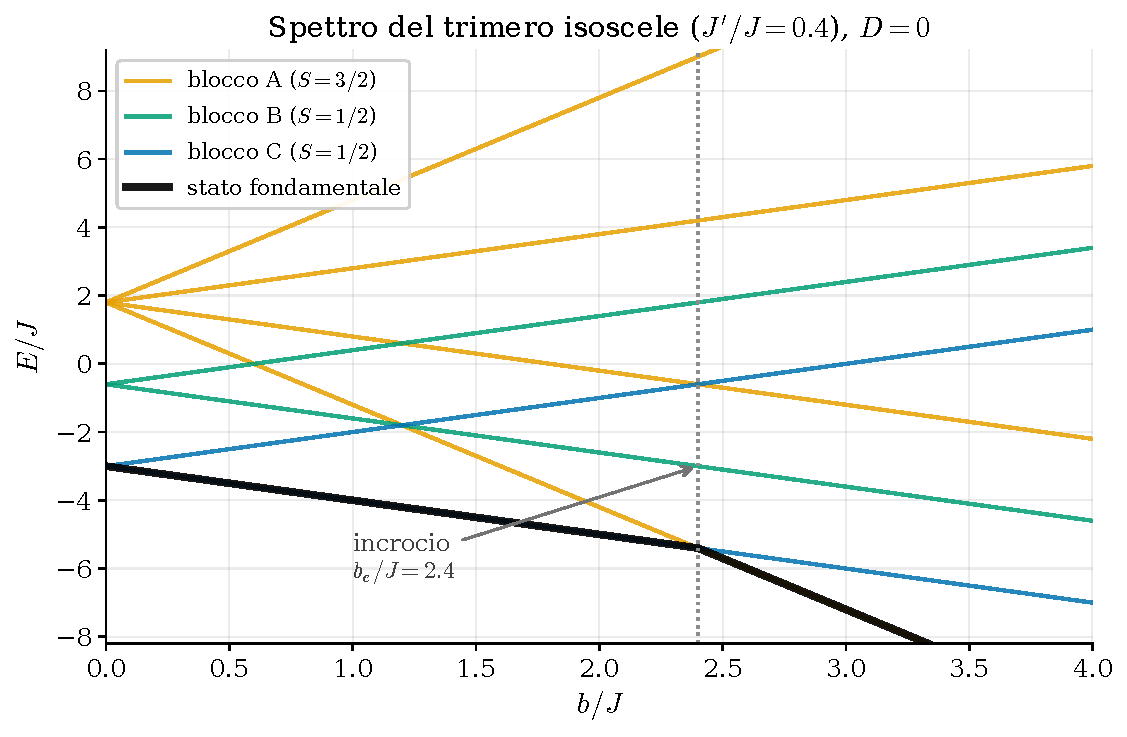
\includegraphics[width=0.82\textwidth]{figure/fig01_spettro_anello}
\caption{Spettro del trimero isoscele ($J'/J=0.4$), $D=0$. Otto livelli in
tre famiglie (blocchi A, B, C secondo la decomposizione di Kambe). La curva
nera segue lo stato fondamentale: dal blocco C, incrocia il blocco A a
$b_c/J=2.4$.}
\label{fig:spettro}
\end{figure}
\FloatBarrier

\verifica{Lo spettro numerico (diagonalizzazione diretta della matrice
$8\times8$) coincide con le formule analitiche dei tre blocchi di Kambe a
precisione macchina, su tutta la griglia in $b$ usata per la
Fig.~\ref{fig:spettro}.}

\section{Perché l'incrocio non si apre da solo}

Stesso argomento di simmetria del dimero, con un ingrediente in più: senza
DM, l'Hamiltoniana conserva sia la magnetizzazione totale $M$ sia
$S_{12}^2$ (il quadrato del momento angolare della coppia base) --- due
numeri quantici buoni, non uno solo. L'incrocio a $b_c$ è fra blocco C
($S_{12}=0$) e blocco A ($S_{12}=1$): stati con $S_{12}^2$ diverso non si
mescolano finché quella simmetria resta intatta, quindi l'incrocio resta
protetto, un incrocio vero.

\section{Il termine DM: due opzioni, effetti opposti}

Qui il trimero si comporta diversamente dal dimero in un modo che vale la
pena vedere esplicitamente: con tre legami, non c'è un solo modo di
accendere un termine DM --- e non è una scelta libera: l'intera teoria del
trimero isoscele assume l'invarianza per scambio dei siti $1,2$
(rappresentata dall'operatore di permutazione $P_{12}$); un DM aggiunto
senza vincoli rischierebbe di rompere quella simmetria in un modo non
giustificato dalla geometria --- un'incoerenza interna con tutto il resto
della teoria costruita sopra quell'ipotesi.

\paragraph{Verifica sistematica, non una scelta a occhio.} Costruito
esplicitamente $P_{12}$ come matrice di permutazione $8\times8$ e
verificato $\|P_{12}H_\text{DM}P_{12}^\dagger-H_\text{DM}\|$ per tutte le
combinazioni di segno di $(D_{12},D_{23},D_{31})\propto(J,J',J')$
(dettaglio completo in \texttt{analisi\_dm\_trimero\_anello.tex}): fra
tutte le disposizioni testate, \textbf{una sola} rispetta esattamente la
simmetria --- nessun DM sul legame di base ($D_{12}=0$), segno opposto sui
due legami laterali equivalenti ($D_{23}=-D_{31}$). Non è una fra le tante
opzioni ugualmente legittime: è l'unica che sopravvive al vincolo.

\begin{itemize}[leftmargin=1.6em,itemsep=3pt]
\item \textbf{Opzione A} (simmetrica): $D_{12}=0$, $D_{23}=-D_{31}=D'$.
Emersa dalla verifica sopra, non scelta a priori. Commuta con $S_{12}^2$
($\|[H,S_{12}^2]\|\sim10^{-16}$, verificato).
\item \textbf{Opzione B} (\emph{proposta del relatore}): $D_{12}=rJ$,
$D_{23}=D_{31}=rJ'$, stesso segno su tutti e tre i legami, proporzionale
allo scambio corrispondente --- una scelta semplice, non derivata dalla
simmetria, suggerita come primo candidato da testare. Rompe la simmetria
$P_{12}$; non commuta con $S_{12}^2$ ($\|[H,S_{12}^2]\|\sim1.4$ a
$r=0.15$).
\end{itemize}

\begin{figure}[htbp]
\centering
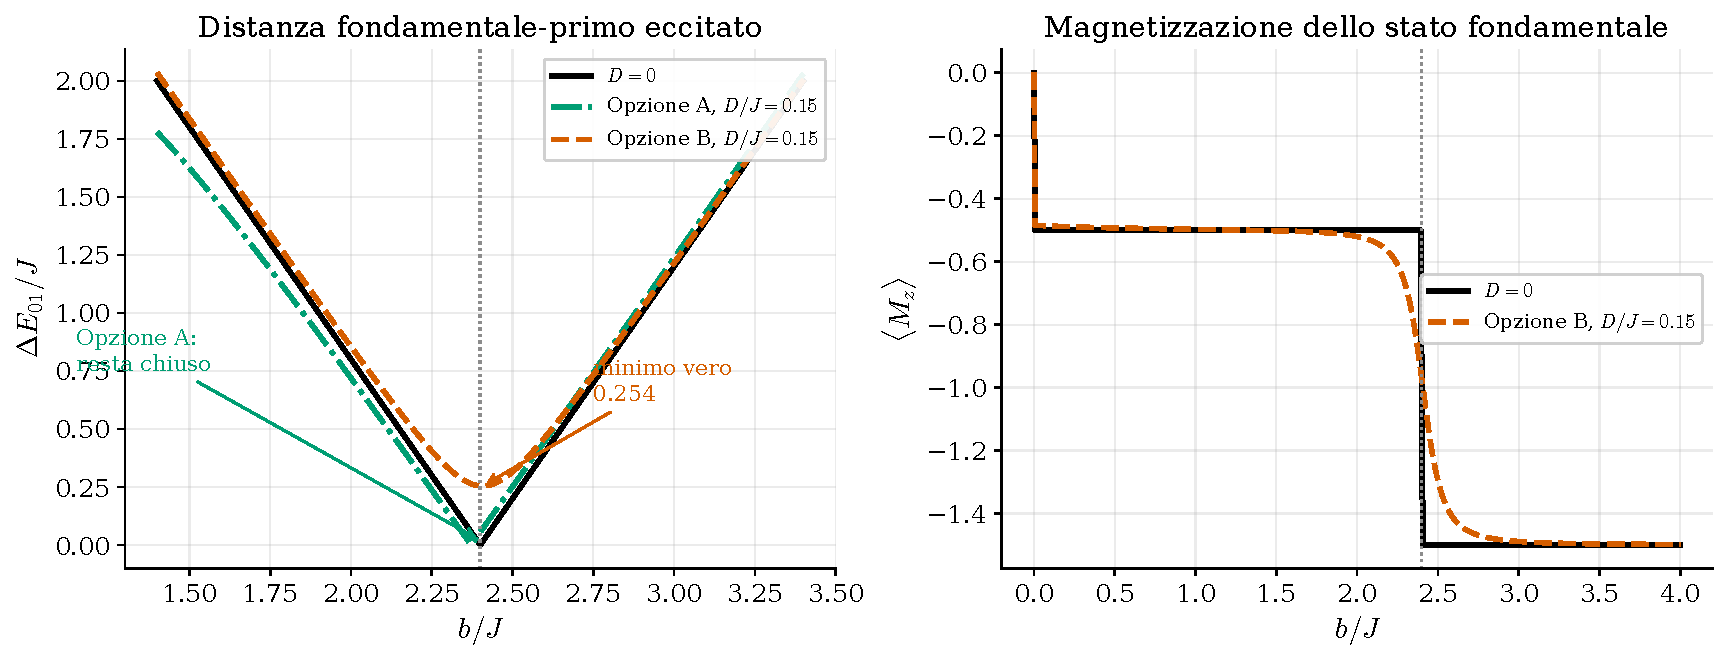
\includegraphics[width=\textwidth]{figure/fig02_gap_magnetizzazione_anello}
\caption{\textbf{A sinistra:} distanza fondamentale--primo eccitato, $D=0$
contro le due opzioni DM ($D/J=0.15$). L'Opzione A (verde) resta
indistinguibile da $D=0$ esattamente al punto critico --- l'incrocio non si
apre. L'Opzione B (rosso) lo apre davvero, gap minimo vero $0.254$, spostato
leggermente a $b/J=2.407$. \textbf{A destra:} magnetizzazione dello stato
fondamentale, $D=0$ contro Opzione B: il salto netto diventa un crossover
continuo, stesso fenomeno del dimero.}
\label{fig:gap}
\end{figure}
\FloatBarrier

\verifica{Gap minimo vero (cercato in un intorno di $b_c$, non a $b_c$
fisso): Opzione A, $2.3\times10^{-8}$ a $b/J=2.372$ --- zero a precisione
numerica, l'incrocio resta chiuso qualunque sia l'intensità del DM in
questa forma. Opzione B, $0.2543$ a $b/J=2.407$. Commutatore con $S_{12}^2$
(norma di Frobenius, come sul dimero): Opzione A, $0$ esatto; Opzione B,
$1.379$ --- diverso da zero, coerente con l'apertura osservata.}

\subsection*{Perché l'incrocio resta vero sotto l'Opzione A: la regola di
non-incrocio di von Neumann--Wigner}

Non è un caso da verificare numero per numero: è una conseguenza diretta
della simmetria. Poiché l'Opzione A commuta con $S_{12}^2$, l'Hamiltoniana
resta a blocchi nei due settori $S_{12}=0$ (blocco C) e $S_{12}=1$
(blocchi A, B) --- l'elemento di matrice fra uno stato C e uno stato A è
\textbf{esattamente zero per ogni $b$}, non solo vicino all'incrocio. La
regola di non-incrocio di von Neumann--Wigner dice che due livelli senza
accoppiamento (stessa simmetria a separarli) possono incrociarsi
liberamente al variare di un solo parametro, senza bisogno di alcun
aggiustamento fine --- è l'assenza di accoppiamento a garantirlo. Sotto
l'Opzione B, che non commuta con $S_{12}^2$, quell'elemento di matrice è
generalmente diverso da zero: la regola non si applica più, e l'incrocio
diventa evitato --- il comportamento standard quando due livelli si
avvicinano senza una simmetria a proteggerli.

\paragraph{Perché il punto dell'incrocio si sposta comunque.} Che
l'incrocio resti vero (Opzione A) non vuol dire che resti \emph{fermo}: la
posizione dipende da dove le energie dei due blocchi si eguagliano, e il
DM può spostare quelle energie anche senza mescolare C con A. Verificato
direttamente sulla struttura a blocchi: sotto l'Opzione A, l'Hamiltoniana
si scompone in un blocco $2\times2$ isolato (il settore $S_{12}=0$, cioè
C --- accoppiamento con il resto verificato nullo, norma $\sim10^{-16}$) e
un blocco $6\times6$ pieno (il settore $S_{12}=1$, dove A e B \emph{si
mescolano fra loro} --- elementi fuori diagonale fino a $1.13$, verificati
esplicitamente). È questo mescolamento A--B, non un semplice spostamento
diagonale, a spingere il ramo più basso del settore $S_{12}=1$ (quello che
diventa il nuovo fondamentale sopra l'incrocio) lontano dalla sua energia
non perturbata --- mentre il blocco C, isolato, resta esattamente fermo
sulla formula $D=0$ per costruzione. Confermato confrontando ciascun ramo
con la formula esatta a $D=0$: il blocco C non si sposta affatto
(differenza nulla a precisione macchina, per ogni $b$ testato); il ramo
più basso del settore $S_{12}=1$ invece sì, di circa $0.05$--$0.08$ a
seconda di $b$. È questo spostamento asimmetrico di un solo settore, non
un mescolamento con C, a spostare il punto d'incrocio da $b/J=2.4$ a
$b/J\approx2.372$.

\verifica{Blocco C--(A+B) fuori diagonale: norma $1.08\times10^{-16}$,
nessun mescolamento con C. Dentro il settore $S_{12}=1$ (6$\times$6):
elementi fuori diagonale fino a $1.13$, A e B genuinamente mescolati.
Lungo il ramo, a $b/J=2.372$: $E_C=-5.372000$, identico alla formula
$D=0$ ($-3J-b$). Ramo più basso del settore $S_{12}=1$: $-5.372352$
contro $-5.316000$ atteso dalla formula non perturbata di A
($J+2J'-3b$) --- differenza $-0.056$: il settore $S_{12}=1$ spostato (per
mescolamento interno A--B), il blocco C no.}

\messaggio{Con un solo legame (dimero) c'è un solo modo di rompere una
simmetria. Con tre legami (trimero) la stessa domanda --- ``il DM apre
l'incrocio?'' --- ha risposte diverse a seconda di \emph{come} il DM è
distribuito sui legami: non basta che il termine sia acceso, conta la sua
forma.}

\section{Perché questo conta per il resto del lavoro}

Stesso ruolo del dimero, con la stessa conseguenza in tre punti:

\begin{enumerate}[leftmargin=1.5em,itemsep=4pt]
\item \textbf{Rende ben posto il problema variazionale}, esattamente come sul
dimero --- ma solo con l'Opzione B: con l'Opzione A l'incrocio resta
degenere, e il VQE al punto critico non avrebbe un bersaglio unico.
\item \textbf{Rompe la simmetria su cui un ansatz efficiente sarebbe
costruito} --- $M$ conservata, non $S_{12}^2$: un ansatz $M$-conservante
(RBS o $W$, Documento 2) può restare confinato in un settore che il vero
fondamentale, con DM acceso, non abita più per intero.
\item \textbf{Impedisce la fattorizzazione esatta dell'evoluzione
temporale} --- con una complicazione in più rispetto al dimero: anche lo
scambio isotropo da solo, con tre legami che condividono qubit, non si
esponenzia in un solo blocco. Il Documento 3 tratta questo aspetto in
dettaglio.
\end{enumerate}

Per il resto della serie si userà sempre l'\textbf{Opzione B}: è l'unica
scelta di DM per cui il trimero riproduce, punto per punto, lo stesso ruolo
che il termine DM ha nel dimero.

\bigskip
\noindent\footnotesize\textit{Riferimento.} Per la decomposizione di Kambe
(composizione dei momenti angolari per sistemi di spin accoppiati): K.~Kambe,
\emph{On the Paramagnetic Susceptibilities of Some Polynuclear Complex
Salts}, J.\ Phys.\ Soc.\ Jpn.\ \textbf{5}, 48 (1950).

\end{document}
